% !TeX encoding = UTF-8

% 载入 SJTUThesis 模版
\documentclass[type=bachelor,language=english]{sjtuthesis}
% 选项
%   type=[doctor|master|bachelor|course],     % 可选(默认:doctor),论文类型
%   zihao=[-4|5],                             % 可选(研究生默认:-4,本科默认:5),正文字号大小
%   language=[chinese|english],               % 可选(默认:chinese),论文的主要语言
%   review,                                   % 可选(默认:关闭),盲审模式
%   [twoside|oneside]                         % 可选(默认:twoside),单双页模式

% 论文基本配置,加载宏包等全局配置
% !TEX root = ./main.tex

\sjtusetup{
  %
  %******************************
  % 注意:
  %   1. 配置里面不要出现空行
  %   2. 不需要的配置信息可以删除
  %******************************
  %
  % 信息录入
  %
  info = {%
    %
    % 标题
    %
    title           = {RISC-V处理器微架构的设计与优化},
    title*          = {RISC-V SoC Design and Optimization},
    %
    % 标题页标题
    %   可使用“\\”命令手动控制换行
    %
    % display-title   = {上海交通大学学位论文\\ \LaTeX{} 模板示例文档},
    % display-title*  = {A Sample Document \\ for \LaTeX-based SJTU Thesis Template},
    %
    % 页眉标题
    %
    % running-title   = {示例文档},
    % running-title*  = {Sample Document},
    %
    % 关键词
    %
    keywords        = {计算机体系结构, 系统级芯片, 嵌入式系统},
    keywords*       = {Computer architecture, System on-chip, Embedded system},
    %
    % 姓名
    %
    author          = {史\quad{}历},
    author*         = {Li Shi},
    %
    % 指导教师
    %
    supervisor      = {钱炜慷},
    supervisor*     = {Prof. Weikang Qian},
    %
    % 副指导教师
    %
    % assisupervisor  = {某某教授},
    % assisupervisor* = {Prof. Uom Uom},
    %
    % 学号
    %
    id              = {517370910032},
    %
    % 学位
    %   本科生不需要填写
    %
    degree          = {工学学士},
    degree*         = {Bachelor of Science in Engineering},
    %
    % 专业
    %
    major           = {电子与计算机工程},
    major*          = {Electrical and Computer Engineering},
    %
    % 所属院系
    %
    department      = {密西根学院},
    department*     = {UM-SJTU Joint Institute},
    %
    % 课程名称
    %   仅课程论文适用
    %
    course          = {VE 450},
    %
    % 答辩日期
    %   使用 ISO 格式 (yyyy-mm-dd);默认为当前时间
    %
    % date            = {2014-12-17},
    %
    % 资助基金
    %
    % fund  = {
    %           {国家 973 项目 (No. 2025CB000000)},
    %           {国家自然科学基金 (No. 81120250000)},
    %         },
    % fund* = {
    %           {National Basic Research Program of China (Grant No. 2025CB000000)},
    %           {National Natural Science Foundation of China (Grant No. 81120250000)},
    %         },
  },
  %
  % 风格设置
  %
  style = {%
    %
    % 本科论文页眉 logo 颜色 (red/blue/black)
    %
    header-logo-color = red,
    title-logo-color = blue,
  },
  %
  % 名称设置
  %
  name = {
    % bib               = {References},
    % acknowledgements  = {谢\hspace{\ccwd}辞},
    % publications      = {攻读学位期间完成的论文},
  },
}

% 使用 BibLaTeX 处理参考文献
%   biblatex-gb7714-2015 常用选项
%     gbnamefmt=lowercase     姓名大小写由输入信息确定
%     gbpub=false             禁用出版信息缺失处理
\usepackage[backend=biber,style=gb7714-2015]{biblatex}
% 文献表字体
% \renewcommand{\bibfont}{\zihao{-5}}
% 文献表条目间的间距
\setlength{\bibitemsep}{0pt}
% 导入参考文献数据库
\addbibresource{bibdata/thesis.bib}

% 定义图片文件目录与扩展名
\graphicspath{{figures/}}
\DeclareGraphicsExtensions{.pdf,.eps,.png,.jpg,.jpeg}

% 确定浮动对象的位置,可以使用[H],强制将浮动对象放到这里(可能效果很差)
% \usepackage{float}

% 固定宽度的表格
% \usepackage{tabularx}

% 表格中支持跨行
\usepackage{multirow}

% 表格中数字按小数点对齐
\usepackage{dcolumn}
\newcolumntype{d}[1]{D{.}{.}{#1}}

% 使用长表格
\usepackage{longtable}

% 附带脚注的表格
\usepackage{threeparttable}

% 附带脚注的长表格
\usepackage{threeparttablex}

% 算法环境宏包
\usepackage[ruled,vlined,linesnumbered]{algorithm2e}
% \usepackage{algorithm, algorithmicx, algpseudocode}

% 代码环境宏包
\usepackage{listings}
\lstnewenvironment{codeblock}[1][]%
  {\lstset{style=lstStyleCode,#1}}{}

% 物理科学和技术中使用的数学符号,定义了 \qty 命令,与 siunitx 3.0 有冲突
% \usepackage{physics}

% 直立体数学符号
\newcommand{\dd}{\mathop{}\!\mathrm{d}}
\newcommand{\ee}{\mathrm{e}}
\newcommand{\ii}{\mathrm{i}}
\newcommand{\jj}{\mathrm{j}}

% 国际单位制宏包
\usepackage{siunitx}

% 定理环境宏包
\usepackage{ntheorem}
% \usepackage{amsthm}

% 绘图宏包
\usepackage{tikz}
\usetikzlibrary{shapes.geometric, arrows}

% 一些文档中用到的 logo
\usepackage{hologo}
\newcommand{\XeTeX}{\hologo{XeTeX}}
\newcommand{\BibLaTeX}{\textsc{Bib}\LaTeX}

% 借用 ltxdoc 里面的几个命令方便写文档
\DeclareRobustCommand\cs[1]{\texttt{\char`\\#1}}
\providecommand\pkg[1]{{\sffamily#1}}

% = = = = = = = = = = = = %
%     JI专用模板调整      %
% = = = = = = = = = = = = %
\usepackage{mwe}
\usepackage{blindtext}
\usepackage{titlesec}
\usepackage{setspace}

% Chapter
\renewcommand\chaptername{\relax}
% \titleformat{\chapter}[hang]{\normalfont\bfseries\LARGE\centering}{\thechapter\quad}{-6pt}{}
% \titlespacing{\chapter}{0pt}{*6}{*3}
% \titleclass{\chapter}{straight}

% Section
\titlespacing{\section}{0pt}{*4}{*1.5}
\titlespacing{\subsection}{0pt}{*4}{*1.5}
\titlespacing{\subsubsection}{0pt}{*4}{*1.5}

% Figure
\renewcommand{\figurename}{Illustration}

% Code
% \usepackage{minted}

% JI Citation formatting
\newcommand{\quickcite} [1] {(\parencite{#1}, \citeauthor{#1}, \citeyear{#1}: \citefield{#1}{pages})}

\newcommand{\quickcitenopage} [1] {(\parencite{#1}, \citeauthor{#1}, \citeyear{#1})}

\newcommand{\quickcitetwo}[2]{(\parencite{#1,#2}, \citeauthor{#1}, \citeyear{#1}: \citefield{#1}{pages}; \citeauthor{#2}, \citeyear{#2}: \citefield{#2}{pages})}

% 自定义命令

% E-mail
\newcommand{\email}[1]{\href{mailto:#1}{\texttt{#1}}}

% hyperref 宏包在最后调用
\usepackage{hyperref}


\begin{document}

%TC:ignore

% 标题页
\maketitle

% 原创性声明及使用授权书
\copyrightpage[scans/ji-copyright.pdf]

% 前置部分
\frontmatter

% 摘要
% !TEX root = ../main.tex

\begin{abstract}
% = = = = = = = = = = = = = = = = = = = %
%               中文摘要                % 
% = = = = = = = = = = = = = = = = = = = %
{
    中文摘要应该将学位论文的内容要点简短明了地表达出来,应该包含论文中的基本信息,体现科研工作的核心思想。摘要内容应涉及本项科研工作的目的和意义、研究方法、研究成果、结论及意义。注意突出学位论文中具有创新性的成果和新见解的部分。摘要中不宜使用公式、化学结构式、图表和非公知公用的符号和术语,不标注引用文献编号。硕士学位论文中文摘要字数为 500 字左右,博士学位论文中文摘要字数为 800 字左右。英文摘要内容应与中文摘要内容一致。
    
    摘要页的下方注明本文的关键词(4~6个)。
}

\end{abstract}

% 1.5倍行距
{
\setstretch{1.5}
\setlength{\parindent}{0pt}
\setlength{\parskip}{1em}

\begin{abstract*}

% = = = = = = = = = = = = = = = = = = = %
%               英文摘要                % 
% = = = = = = = = = = = = = = = = = = = %
{
    \blindtext
}

\end{abstract*}

}

% 目录
\tableofcontents

%TC:endignore

% 主体部分
\mainmatter

% 正文内容
{
\setstretch{1.5}
\setlength{\parindent}{0pt}
\setlength{\parskip}{1em}

% = = = = = = = = = = = = = = = = = = = = = %
%                  Chapters                 %
% = = = = = = = = = = = = = = = = = = = = = %

% !TEX root = ../main.tex

% = = = = = = = = = = = = = = = = = = = %
%             Introduction              % 
% = = = = = = = = = = = = = = = = = = = %

\let\clearpage\relax
\chapter{Introduction}

\section{Figures}

\subsection{Single Figure}

\begin{figure}[!htp]
    \centering
    \includegraphics[scale=0.5]{example-image-a}
    \caption{Figure-A.}
    \label{fig:a}
\end{figure}

\subsection{Subfigures}

\begin{figure}[!htp]
    \begin{minipage}{0.48\textwidth}
        \centering
        % include first image
        \includegraphics[scale=0.5]{example-image-a}
        \caption{Subfigure-A.}
        \label{fig:sub_a}
    \end{minipage}\hfill
    \begin{minipage}{0.48\textwidth}
        \centering
        % include second image
        \includegraphics[scale=0.5]{example-image-b}
        \caption{Subfigure-B.}
        \label{fig:sub_b}
    \end{minipage}
\end{figure}

\section{Table}

\begin{table}[!htp]
    \begin{center}
    \caption{Table-1.}
    \label{tab:tab-1}
        \begin{tabular}{cc}
            \toprule
                Item   &   Value \\
            \midrule
                A      &   1,000 \\
                B      &   2,000 \\
                C      &   3,000 \\
            \bottomrule
        \end{tabular}
    \end{center}
\end{table}

\section{Citation}

Single document with available page number~\quickcite{kopka1995guide}.

Single document without available page number~\quickcitenopage{kottwitz2015latex}.

Two documents at the same time~\quickcitetwo{lamport1985i1}{kopka1995guide}.

\section{Source Code}

\subsection{Pseudocode}
\begin{algorithm}
\caption{Algorithm 1.}
\label{alg:alg-1}
    \KwIn{integers $a,b$}
    \KwOut{integers $c$}
    \If {$a > b$} {
        $c = a - b$ \;
        \tcp{This is a comment.}
    }
    \Else {
        $c = a + b$ \;
    }
\end{algorithm}

\subsection{Source Code}

\begin{minted}[mathescape,
               linenos,
               numbersep=5pt,
               gobble=2,
               frame=lines,
               framesep=1mm]{python}
    def my_function():
        print("Hello from a function")
\end{minted}
% = = = = = = = = = = = = = = = = = = = = = %
%              Specifications               %
% = = = = = = = = = = = = = = = = = = = = = %

\let\clearpage\relax
\chapter{Customer Requirements \& Engineering Specifications}

\section{Customer Requirements (CR)}
Since our project is experimental and research-oriented, there do not exist specific customers for our design. However, customer requirements are still necessary, as after the completion of our project, potential embedded system customers may be interested. Meanwhile, mainstream CPU and SoC evaluation indices still apply to our design, e.g., core frequency, performance, energy efficiency, power consumption, etc. Briefly speaking, our target market is artificial intelligence hardware systems, and the consumers include users who want to run machine learning applications in their embedded systems.

We divide our customer requirements into three categories: general (G), performance (P), and embedded system (ES). For the general part, customers may require that the design should be compatible to general RISC-V applications, and attached with clear documentations. Target users of our design may include computer science researchers, embedded system users, or both. The former requires the performance part, e.g., good performance for machine learning applications, and the latter requires the embedded system part, e.g., low power consumption and quick response.


\subsection{General Requirements}
The main concern for the general requirements part is to set up proper constraints so that we can achieve good compatibility as well as usability. This is determined by the characteristics of our target market and consumers.

The target market of our SoC is a sub-division of the traditional computing hardware market, which requires tight constraint on performance, cost and energy efficiency. Thus, the general requirement should be a super-set of current computing market. For example, microprocessors and computing system based RISC-V ISA has solid ecosystem and active community. Tool chains like \texttt{gcc} compiler support, Linux kernel support and verification support are well established \cite{rvsoftware}. The market will welcome a new SoC which is fully compatible with current RISC-V ecosystem because the cost to adopt our product will be low and they will need fewer labors and less time, comparing to the product needs software part from scratch. Also, the competitive computing market requires good usability to win the business. The computing hardware market requires good documentations, as experienced engineers in this high standardized industry can be much more productive when the documentation follows professional protocols. This requirement can also be justified if we consider who is our target consumers. It is hard for startups or small size company to use our product because these companies generally cannot take the risk to adopt a new SoC. Our target consumer will be medium or large size, system level companies who want to use our SoC to increase their current product's efficiency. These companies have strong low-level research and development capability, and their software or application may be architectural specific. Therefore, they will prefer a new SoC with minimum architectural change and requires little effort to deploy their applications. Compatibility and usability are therefore the main points in the General requirements part.

As our SoC is based on the RISC-V architecture, being compatible with the RISC-V architecture is the most important constraint to consider. RISC-V is a family of ISA, so selecting a proper RISC-V ISA subset is critical. RISC-V ISA includes a base integer ISA, like RISC-V 32I, and optional extension to the base ISA. We want our SoC to be a stable target for RISC-V applications so that the application source code written in high level language like C/C++ can be correctly mapped to our SoC. To run general RISC-V applications, a RISC-V 32G is a reasonable target as suggested by the RISC-V specification \cite{RISC-V_unprivileged_ISA}, which includes:
\begin{enumerate}
    \item RISC-V 32I base ISA
    \item RISC-V M extension, for integer multiplication and division
    \item RISC-V A extension, for atomic instructions
    \item RISC-V F extension, for single-precision floating-point
    \item RISC-V D extension, for double-precision floating point
\end{enumerate}

RISC-V 32G applications encode their instructions in 32 bits. However, due to the limited memory size of many embedded systems, we hope that the size of applications can be as small as possible. One of the solutions is to introduce RISC-V C extension for compressed instructions, where instructions are encoded in 16 bits. If time permits, we should add the support for RISC-V C extension to further optimize for embedded systems.

To enhance the usability of our SoC, a clear and clean documentation is needed. Enough documentation should be written for each module, each subsystem and the overall design. If time permits, some performance analysis can also be added in the documentation so the consumers can better unleash the potential of our SoC.

Finally, due to the requirement of cost control in most embedded system designs, our SoC should be as inexpensive as possible.

\textbf{General Requirements:}
\begin{enumerate}
    \item Is compatible with RISC-V applications (weight: 10)
    \item Has good documentation for reference (weight: 6)
    \item Is inexpensive (weight: 5)
\end{enumerate}


\subsection{Performance Requirements}
While Gordon Moore predicted the growth in semiconductor, he also foresaw its end 50 years later. In recent days, even the company uses Moore's law as a guideline have to slow their pace to build even smaller transistor. Therefore, our SoC faces a market which require smart design to achieve higher performance under current technology node.
The market will first need high performance for normal arithmetic operations. Although nowadays specific AI algorithms rely heavily on the matrix operations, the normal arithmetic operations still take great part in a program to do branching, jumping, indexing, etc. Thus, to achieve an overall high performance, we need to have high performance normal arithmetic units and designs so that this part will not be a bottleneck. For the normal operations, the performance throughput equals to frequency times the Instructions executed per clock cycle (IPC). In order to achieve a high throughput, we need both a high frequency and a high IPC. Designing more pipeline stages may help achieve higher clock frequency, but may result in higher plenty when there is a miss prediction. Dynamic scheduling is a technique to increase the throughput by enabling Out-of-Order execution when instructions have no dependency. This method extract instruction level parallelism and it is always combined with other technique like renaming, speculative execution to  maximize the outcome. Also, enough number of function unit is needed so that the pipeline will not stall during the congestion at the execution stage. Our SoC should adopt these traditional techniques to have a high performance on the traditional normal arithmetic operations.

The AI application is a hot topic today. The performance for running AI application is also demanded by our target market. One of the most significant properties of this application is that it is error torrent. During the inference, minor error will not introduce much difference on the final result. During the training, some error may even manually be introduced to increase the robustness of the algorithm. This makes approximate computing a potential way to achieve higher frequency by using circuits with fewer elements.

Another property of AI application is that it is data driven, which means it is usually memory-bounded. Our SoC needs a high performance memory subsystem to make sure the pipeline for AI application will not hungry for data and halt. By using memory hierarchy and introducing cache, we can exploit the temporary locality and spacial locality of memory access to increase the memory subsystem's performance. One of the most important parameter that determines the cache's performance is its size. A trade off between the cache size and other parameter like frequency needs to be made so that the overall performance can be improved.

Before our design is fixed, we want do some architecture exploration. Therefore, we want the parameters of some of the critical modules, like the reorder buffer size and cache size is configurable so that we can change them to evaluate performance.

\textbf{Performance Requirements:}
\begin{enumerate}
    \item Runs fast for normal arithmetic operations (weight: 8)
    \item Runs fast for machine learning applications (weight: 9)
    \item Runs fast for memory-bound applications (weight: 7)
    \item Can be configured with different parameters (weight: 2) % this should not be a ES requirement as it happens before design was fixed.
\end{enumerate}


\subsection{Embedded System Requirements}
Although the ware-house scale computing center still take plenty of the computation nowadays, the market has a trend to offload part of the computation to the edge because of security issue, latency issue, etc. Our SoC will be more competitive at the edge as the concept AI on things has attracted lots of attention. Therefore, we require our SoC satisfy some requirement for embedded system.

The embedded system is often energy-bounded as the power source is usually a battery. High power consumption is not allow because these scenario often require long battery life. The can be evaluated using the number of operations processed within unit energy, so our SoC should have a limited number at this part. Some embedded system also have requirement on latency. For AR/VR application, this requirement is necessary as longer latency will cause discomfort. We hope our SoC can provide a low average response time to a request for service. The market also requires embedded SoC have low cost, as the embedded system application is normally cost sensitivity. This can be evaluated by the usage of resources on the FPGA, like look-up tables (LUTs), block RAMs (BRAMs) and digital signal processors (DSPs). The embedded system also has to need to connect to various types of peripherals, so have more I/O controllers can make our product more competitive on the market.

\textbf{Embedded Requirements:}
\begin{enumerate}
    \item Saves power (weight: 6)
    \item Responds quickly (weight: 4)
    \item Low cost (weight: 3)
    \item Has good support for multiple I/O devices (weight: 3)
\end{enumerate}


\subsection{Benchmark Competitions against CR}
In this part, we quickly review some existing open-source solutions against customer requirements. This step gives us a better view of customer requirements as well as offers us some clue on how to design our own products based on existing solutions.

The evaluation is based on a 5-point scale, where 5 means ``satisfies perfectly'' and 1 means ``doesn't satisfy at all''. We select four open-source solutions to evaluate: MIPS processor with classical 5-stage pipeline, Rocket Core, Berkeley Out-of-Order Machine (BOOM), and Hummingbird E203. For instance, in terms of ``is compatible to general RISC-V applications'', we find that Rocket Core and BOOM have the best support, so we give them 5 points. Hummingbird E203 has limited support for RISC-V applications, so we give it 3 points. The MIPS processor with classical 5-stage pipeline is not compatible with RISC-V applications, so we give it 1 point.

The detailed benchmark competitions against CR are shown in the HOQ chart (Fig. \ref{qfd}).


\section{Engineering Specifications (ES)}
Based on the previous customer requirements, we come up with our engineering specifications of our project, which represent for the quantifiable measures to guide us to design the project properly that can meet customers' requirements. Table \ref{es} shows our overall engineering specifications in our project design.

\begin{table}[!htp]
\centering
\begin{tabular}{lcc}
\hline
\textbf{Engineering Specification} & \textbf{Unit} & \textbf{Target Value} \\
\hline
Support RV32G instruction set architecture (ISA) & -     & Yes          \\
Core frequency on FPGA test platform             & MHz   & 100          \\
Number of pipeline stages                        & -     & 9            \\
Instructions executed per clock cycle (IPC)      & -     & 0.5          \\
Support instruction dynamic scheduling           & -     & Yes          \\
Typical total cache size                         & KB    & 32           \\
Number of function units                         & -     & 6            \\
Average response time to a request for service   & ms    & 10           \\
Usage of look-up tables (LUT) on FPGA            & k     & 120          \\
Usage of block RAM (BRAM) on FPGA                & -     & 50           \\
Usage of digital signal processor (DSP) on FPGA  & -     & 30           \\
Power consumption on target FPGA test platform   & W     & 5            \\
Operations processed within unit energy.         & MOp/J & 25           \\
Number of flexibly-configured modules            & -     & 10           \\
Number of I/O device types                       & -     & 3            \\
User guide and programmers manual                & -     & Yes          \\
\hline
\end{tabular}
\caption{Engineering specifications.}
\label{es}
\end{table}

This should be a key step to ``translate'' customers' words into professional terms and specifications. For instance, when customers require that their RISC-V applications can run on our SoC, what we actually need is that our SoC should support RV32G ISA. In this part, we will explain how we check the cross correlation of ES, examine the benchmark competitions against ES, set our own target for ES, and most importantly, correlate CR to ES.


\subsection{Cross Correlation of ES}
In this step, we check the cross correlation of ES, and reveal some internal connection between each specification we just made in the previous step. For example, when we increase the number of function units, the usage of hardware resources also increases. When we want to support instruction dynamic scheduling to support out-of-order instruction execution, we can greatly improve the number of instructions executed per clock cycle, which is a significant mark of performance improvement.

This step also gives us a clear guidance on design trade-offs. The most evident contradiction is that the SoC we want to design can never achieve low cost, high performance, low power consumption at the same time, which exactly corresponds to our three different parts of customer requirements. For example, if we want to improve the performance, possible solutions include increasing the frequency, increasing the number of function units, etc., none of which is good for saving power and reducing cost.


The detailed cross correlation of ES is given in the HOQ chart (Fig. \ref{qfd}).


\subsection{Benchmark Competitions against ES \& Set Target for ES}
It is important to perform some benchmark on some existing solutions in terms of our engineering specifications, which enables us to understand better about drawbacks of existing solutions as well as our design targets in the future.

This process sometimes requires ``reverse engineering'' for commercial products, but should be much easier for open-source products. In our survey, except that Hummingbird E203 is partially open-source, all the other three processors are completely open-source, and we should be able to access the data conveniently. However, we need to pay attention that some data is still difficult to access, e.g., the average response time to a request for service. There are some reasons for this kind of lack of data. First, even though the processor design is open-source, the synthesis tool or the test suites are not open-source, leading to the difficulty to reproduce the test results. Second, even though the test processes are completely public, the results may depend on the specific hardware testing platform, which may be expensive or inaccessible. Third, some of the designs can be flexibly configured, and there is no standard or typical settings, as a result of which the test results under different settings can not be referred or compared directly.

In this step, we try our best to explore the data of these existing solutions. Some data can be easily accessed, e.g., the number of pipeline stages or whether instruction dynamic scheduling is supported, while some other data cannot. \cite{processor_benchmark} provides us with many useful indicators to evaluate a design and meanwhile gives us lots of data of both Rocket Core and BOOM, including usage of hardware resources, etc.

Based on the data of existing solutions, we come up with our target values for ES. For example, as our aim is to provide good experience for machine learning application users, performance is crucial to some applications like neutral network, and hence we decide to support instruction dynamic scheduling, and set a relatively high value of core frequency of our design. During the process of deciding our own targets, we mainly refer to the data of BOOM, but also look at the data of other three solutions.

The detailed benchmark competitions against ES and our targets for ES are shown in the HOQ chart (Fig. \ref{qfd}).

\subsection{Correlation from CR to ES}
In this step, we not only make our engineering specifications from scratch, but also check whether all the customer requirements can be covered in our specifications. While the following paragraphs give a short explanation on how we transform CR into ES.

\begin{enumerate}
    \item \textbf{General part}: As customers require that our SoC should be compatible to general RISC-V applications, we require that our SoC should support RV32G ISA. As customers need good and clear documentation, we require that we need to deliver SoC user guide and programmer manual. To control the cost, we need to control our circuit size by limiting our usage of hardware resources, e.g., usage of look-up tables (LUT), digital signal processors (DSP), and block RAMs (BRAM).
    \item \textbf{Performance part}: We want to optimize our SoC for three different customer scenarios: normal arithmetic operations, machine learning applications, and memory-bound applications. They share some common characteristics, e.g., they all require that our SoC should support instruction dynamic scheduling and as high core frequency as possible. Meanwhile, they differ in some specific aspects. For instance, as normal arithmetic applications and machine learning applications are mostly compute-bound, they will benefit more from the improvement on core frequency, instructions executed per clock cycle, and number of function units, while memory-bound applications will benefit more from the improvement on total cache size, as cache is used to accelerate the access to memory.
    \item \textbf{Embedded system part}: Customers require that our SoC works well in embedded systems. To save power, we need to monitor and control the power consumption and energy efficiency of our SoC. To achieve quick response, we need to measure the average response time to a request for service. To configure our SoC with different parameters easily, we need to increase the number of flexibly-configured modules in our digital design. To have good support for multiple I/O devices, we need to support multiple kinds of I/O types and test on various I/O devices.
\end{enumerate}

\section{Quality Function Development (QFD)}
We develop our House of Quality (HOQ) chart with QFD method. The HOQ chart is shown in Fig. \ref{qfd}.

\begin{figure}[!htp]
    \centering
    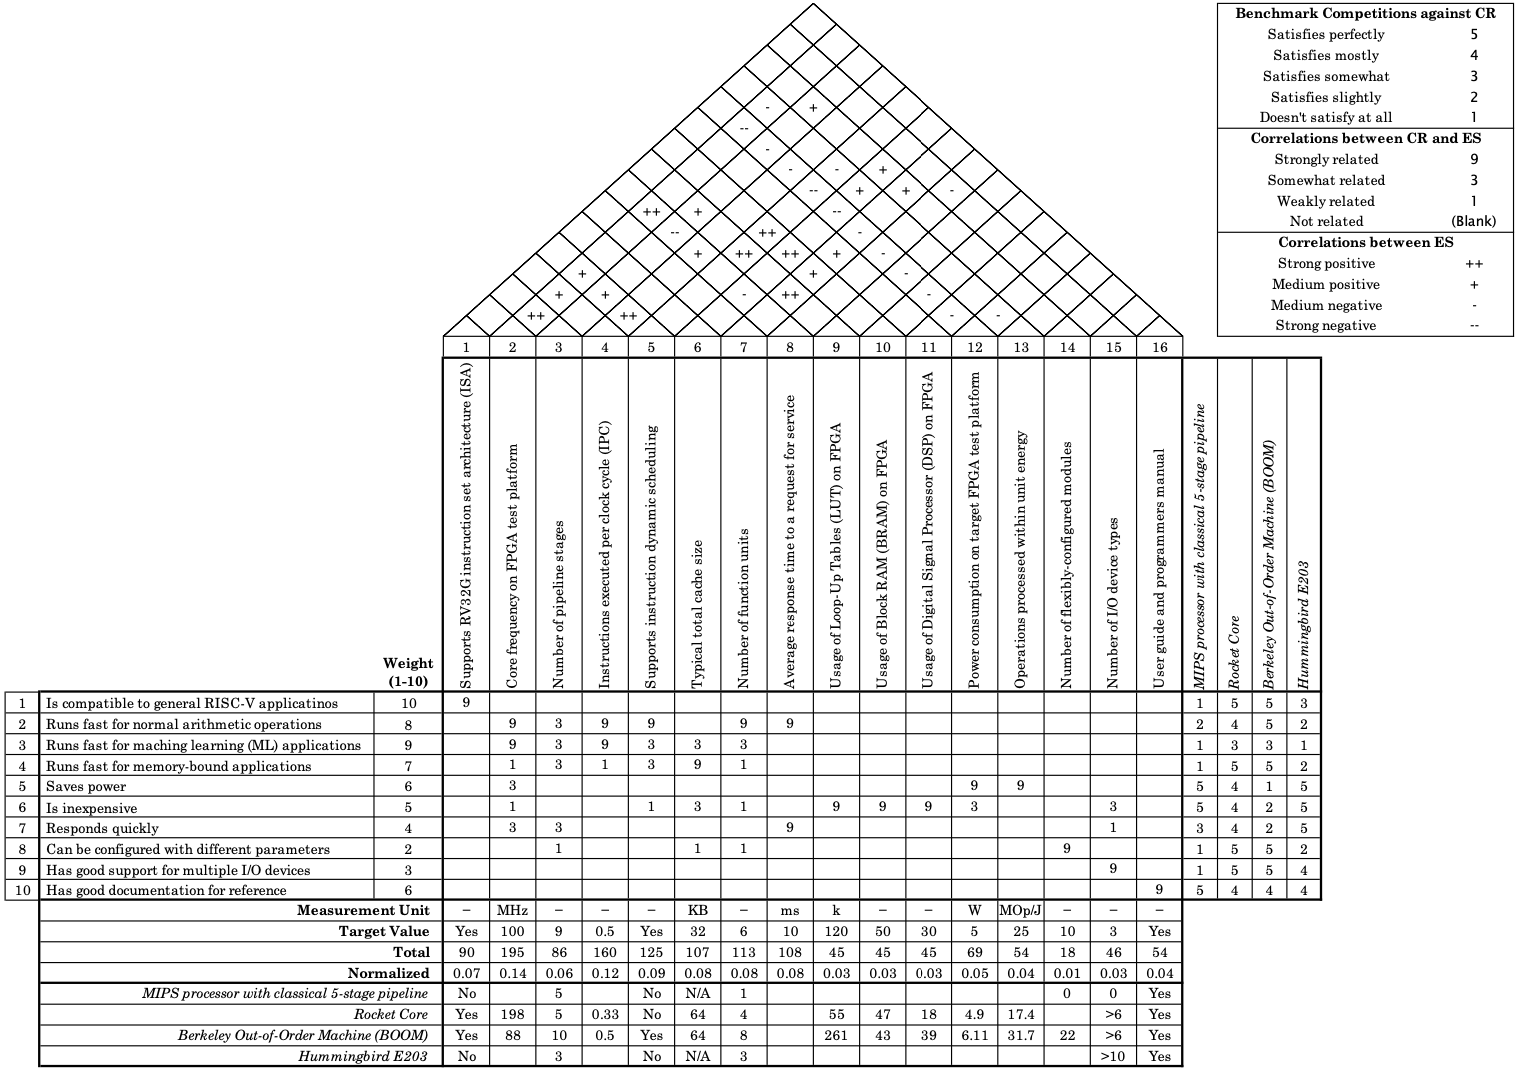
\includegraphics[width=\linewidth]{figure/qfd.png}
    \caption{House of Quality (HOQ) chart.}
    \label{qfd}
\end{figure}

The main steps of QFD method has been expanded in the previous sections. Finally we are able to examine our design priority according to ``Total'' and ``Normalized'' fields. The top 5 engineering specifications we need to consider are core frequency, instructions executed per clock cycle, support for instruction dynamic scheduling, number of function units, and average response time. The result generally matches our expectation that performance is still among the most important factors in embedded system SoC design. Meanwhile, some specifications like number of flexibly-configured modules are relatively not as important as previous ones.

% = = = = = = = = = = = = = = = = = = = = = %
%                  Concept                  %
% = = = = = = = = = = = = = = = = = = = = = %

\let\clearpage\relax
\chapter{Concept Selection}

\blindtext
% = = = = = = = = = = = = = = = = = = = = = %
%             Design Description            %
% = = = = = = = = = = = = = = = = = = = = = %

\let\clearpage\relax
\chapter{Design Description}

\blindtext
% = = = = = = = = = = = = = = = = = = = = = %
%                 Manufacture               %
% = = = = = = = = = = = = = = = = = = = = = %

\let\clearpage\relax
\chapter{Manufacture and Validation}

\blindtext
% = = = = = = = = = = = = = = = = = = = = = %
%                   Results                 %
% = = = = = = = = = = = = = = = = = = = = = %

\let\clearpage\relax
\chapter{Results}

\blindtext
% = = = = = = = = = = = = = = = = = = = = = %
%                 Conclusion                %
% = = = = = = = = = = = = = = = = = = = = = %

\let\clearpage\relax
\chapter{Discussions and Conclusion}

\blindtext

}

%TC:ignore

% 致谢
% !TEX root = ../main.tex

\begin{acknowledgements}

Thanks to \href{https://github.com/sjtug/SJTUThesis}{\sjtuthesis~Team} for providing the \LaTeX~template for this thesis document.

\end{acknowledgements}


% 附录
\appendix
{
\setstretch{1.5}
\setlength{\parindent}{0pt}
\setlength{\parskip}{1em}
% \renewcommand{\thechapter}{\Roman{chapter}}
\captionsetup{list=no}

% = = = = = = = = = = = = = = = = = = = = = %
%                  Appendix                 %
% = = = = = = = = = = = = = = = = = = = = = %

% = = = = = = = = = = = = = = = = = = = = = %
%                    Bios                   %
% = = = = = = = = = = = = = = = = = = = = = %

\chapter{Bios}

\section{Mou Mou}
\begin{minipage}{0.25\textwidth}

\includegraphics[width=1.2in,height=1.5in,clip,keepaspectratio]{example-image-a}

\end{minipage}
\begin{minipage}{0.75\textwidth}\raggedright

\begin{tabular}{l l}
\textbf{Affiliation} & \texttt{B.S. ECE at UM-SJTU JI} \\
\textbf{Stud. ID.} & \texttt{517370910000} \\
\textbf{Email} & \url{jaacount@sjtu.edu.cn}\\
\textbf{Phone} & \texttt{+86 23333333333}\\
\textbf{Programming} & \texttt{Python, C/C++, Matlab} \\
\textbf{Skills} & \texttt{Paddling, Fish Touching}
\end{tabular}

\end{minipage}

\paragraph{Short Bio}
\blindtext

\paragraph{Future Plan}
\blindtext

% = = = = = = = = = = = = = = = = = = = = = %
%                  Appendix                 %
% = = = = = = = = = = = = = = = = = = = = = %

\chapter{Engineering Changes Notice (ECN)}

\begin{figure}[!htp]
    \centering
    \includegraphics[scale=0.5]{example-image-a}
    \caption{Figure-A.}
    \label{fig:a}
\end{figure}


}

% 结尾部分
\backmatter

% 参考文献
\printbibliography[heading=bibintoc]

% 个人工作报告
{
\setstretch{1.5}
\setlength{\parindent}{0pt}
\setlength{\parskip}{1em}

% = = = = = = = = = = = = = = = = = = = = = %
%                Individual                 %
% = = = = = = = = = = = = = = = = = = = = = %

\copyrightpage[scans/report-cover.pdf]
\addcontentsline{toc}{chapter}{Individual Contribution Reports}
\chapter*{Li Shi's Individual Contribution Report}

\blindtext

\section*{Contributions}

\blindtext

\section*{Inspiration and Exploration}

\blindtext

\section*{Skills and Knowledge Acquisition}

\blindtext

}

%TC:endignore

\end{document}
